\subsection{Capa física}
El estándar de CAN define el bit enconding, el timing, y la sincronización. La capa física es la encargada de convertir 1 y 0 en pulsos eléctricos para enviar mensajes por el canal, y también el proceso inverso cuando recibe mensajes. La capa física es implementada enteramente en \ac{HW} \citep{texasFISICACAN}.

\subsubsection{Bus de comunicación}
Para iniciar una transmisión de mensaje es necesario como mínimo dos nodos conectados al bus CAN. Esto se debe a que el dispositivo que envía un mensaje está también recibiendo su propio mensajes, con esto puede chequear cada bit que ha enviado. De esta manera, un segundo nodo responde un un ACK mientras el bit todavía está siendo transmitido por el primer nodo. Esto demuestra por qué se necesitan de dos nodos para completar la transmisión de mensajes \citep{texasFISICACAN}.

En la Figura \ref{fig:traficBUSCAN} se observa un ejemplo extraído de \citep{texasFISICACAN}. En esta se muestra un nodo A que envía un mensaje. Luego se ve que que B y C contestan con un ACK indicando que el mensaje fue recibido sin errores. Luego B y C comienzan a transmiti hata que C gana el bus debido a que tiene un bit dominante, y termina este completando su mensaje.

\begin{figure}[h]
 \centering
 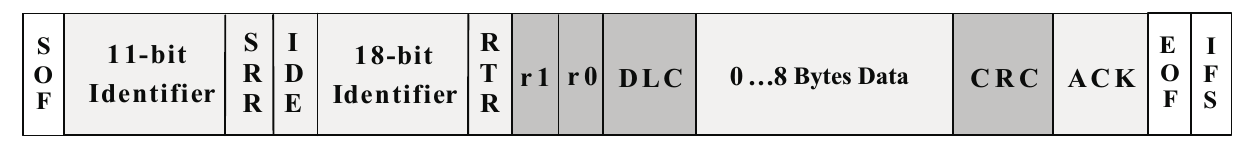
\includegraphics[scale=0.3]{images/Marco_teorico/ExtendedCAN.png}
  \caption{Tráfico en el BUS CAN}
\label{fig:traficBUSCAN}
\end{figure}

El médio físico  es una línea de bus con dos cable, terminada por una resistencia. Los cables pueden ser paralelos, trenzados y/o blindandos. Los segmentos de cable para la conexión de los nodos deben ser lo más cortos posibles.

Para mayores detalle técnico referentes al bus será necesario estudiar el estándar ISO 11898 o en \cite{texasFISICACAN}.

El largo del bus va a determinar el bitrate de la comunicación. Para alcanzar un bitrate de 1Mbps el máximo del canal de comunicación es de 40m. Si se tiene un bus de 1km el bitrate es de 0.05Mbps. Con esto se puede observar que el bitrate decae cuando la distancia se incrementa. Para el CAN el bitrate también está determinado por el total del delay del sistema \citep{texasFISICACAN}. Esto es la suma de los delays del nodo, y el delay propio del cable.

Debe destacarse qde que existen diferentes capas físicas para el protocolo CAN:
\begin{itemize}
\item El tipo más común es el establecido en el estanar ISO 11898-2. Este protocolo cuenta con dos cables, cada uno identificado como CAN\_H y CAN\_L. También es llamado \textit{CAN de alta velocidad} (1 Mbit/s). Este requiere que el alrgo del cable sea como máximo 40m.
\item También en el estándar de ISO se estable el ISO 11898-3, el cual define otro esquema de doble cable balanceado pero para bajas velocidades. Este es tolerante a fallas si alguno de los cables entra en corto circuito. Este es llamado también como \textit{CAN de baja velocidad} (125 kbit/s)
\item Se define el SAE J2411 que utiliza un solo cable para la capa física. Este es utilizado en autos (velocidad por encima de los 50 kbit/s). No tiene demasiados requerimientos en cuanto al bitrate ni el largo del canal de comunicación. EL estandar define 32 nodos por red.
\item Existen modificaciones del estandar RS485 para su funcionamiento con CAN
\end{itemize}

\subsubsection{Bit timing}
El tipo de señal es codificado con Non Return Zero (NRZ). Los bits son codificados en dos estados llamados ``recesivo'' y ``dominante''(el bit 0 es asociado al bit dominante). El protocolo pemite acceso al bus multi-master con una resolución determinística ante colisiones. Para lograr la sincronización, el protocolo sincroniza durante las transiciones. Por tal motivo, deben evitarse el envío de largas cadenas de bits en un mismo estado. CAN utiliza una técnica que se denomina ``bit stuffing'' o ``bit padding'' en la cual luego de enviar 5 bits con el mismo estado, se insertan bits de relleno.

\subsubsection{Asignación eficiente del bus}
La asignación del bus depende de su aplicación. Generalmente existen 2 tipos de clases de asignación.

\begin{itemize}
\item \textbf{Asignación en un tiempo fijo}: La asignación se hace secuencialmente a cada participante sin importar si este necesita el bus en ese momento. Esta técnica, asigna tiempo del bus a cada nodo, y si no tiene nada que enviar, el bus se encuentra ocioso.

\item \textbf{Asignación en base a sus necesidades}: el bus se asigna según las necesidades del nodo (utilizando CSMA o CSMA/CD). En CAN la asignación del bus es negociado entre los mensajes que esperan ser transmitido. CAN utiliza esta técnica.
\end{itemize}
